\begin{figure}[!h]
\centering
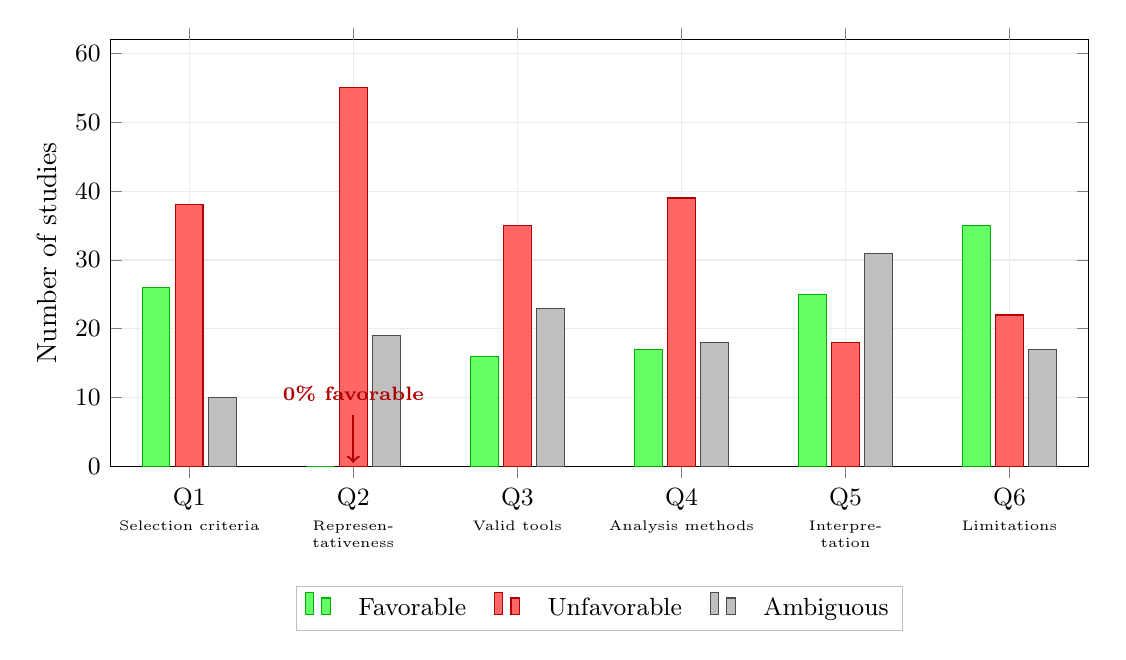
\begin{tikzpicture}
\begin{axis}[
    ybar,
    width=14cm,
    height=7cm,
    ylabel={Number of studies},
    ymin=0, ymax=62,
    symbolic x coords={Q1,Q2,Q3,Q4,Q5,Q6},
    xtick=data,
    xticklabel style={font=\small},
    yticklabel style={font=\small},
    bar width=0.35cm,
    enlarge x limits={abs=1cm},
    legend style={at={(0.5,-0.28)}, anchor=north, legend columns=3,
        font=\small, draw=gray!50, column sep=8pt, /tikz/every even column/.append style={column sep=8pt}},
    grid=major,
    grid style={gray!15, thin},
    ytick={0,10,20,30,40,50,60},
    % Extra x-axis labels below the Q codes
    extra x ticks={Q1,Q2,Q3,Q4,Q5,Q6},
    extra x tick style={
        xticklabel style={font=\tiny, anchor=north, yshift=-12pt, text width=2cm, align=center},
    },
    extra x tick labels={
        {Selection criteria},
        {Represen-\\tativeness},
        {Valid tools},
        {Analysis methods},
        {Interpre-\\tation},
        {Limitations}
    },
]
% Favorable (green)
\addplot[fill=green!60, draw=green!70!black] coordinates {
    (Q1, 26) (Q2, 0) (Q3, 16) (Q4, 17) (Q5, 25) (Q6, 35)
};
% Unfavorable (red)
\addplot[fill=red!60, draw=red!70!black] coordinates {
    (Q1, 38) (Q2, 55) (Q3, 35) (Q4, 39) (Q5, 18) (Q6, 22)
};
% Ambiguous (gray)
\addplot[fill=gray!50, draw=gray!60!black] coordinates {
    (Q1, 10) (Q2, 19) (Q3, 23) (Q4, 18) (Q5, 31) (Q6, 17)
};
\legend{Favorable, Unfavorable, Ambiguous}
% Callout annotation for Q2
\node[font=\scriptsize\bfseries, text=red!70!black, anchor=south] at (axis cs:Q2, 8) {0\% favorable};
\draw[->, thick, red!70!black] (axis cs:Q2, 7.5) -- (axis cs:Q2, 0.5);
\end{axis}
\end{tikzpicture}
\caption{Signalling question-level analysis of risk-of-bias assessments across 74 studies. Q2 (sample representativeness) received no favourable ratings --- the single most striking methodological finding in the corpus. Q6 (limitations discussed) achieved the highest favourable rate (47.3\%) (see Section~\ref{sec:rob-results}).}
\label{fig:signalling-questions}
\end{figure}
